\chapter{Обгрунтування методології проектування та постановка задачі}
\label{chap:second}

\section{Обгрунтування методології проектування та функціональна модель задачі}

Методологією проектування обрана модель waterfall, тому що предметна область не відрізняється високою динамікою на ринку а тому і в плані вимог. Обрана модель забезпечує оптимальний процесс створення системи.

Стандартом за яким проводиться опис ІС було обрано UML, середовище UML Designer 9.0

Функціональна модель системи наведено нище:

TODO: UML UseCase diagram

\begin{center}

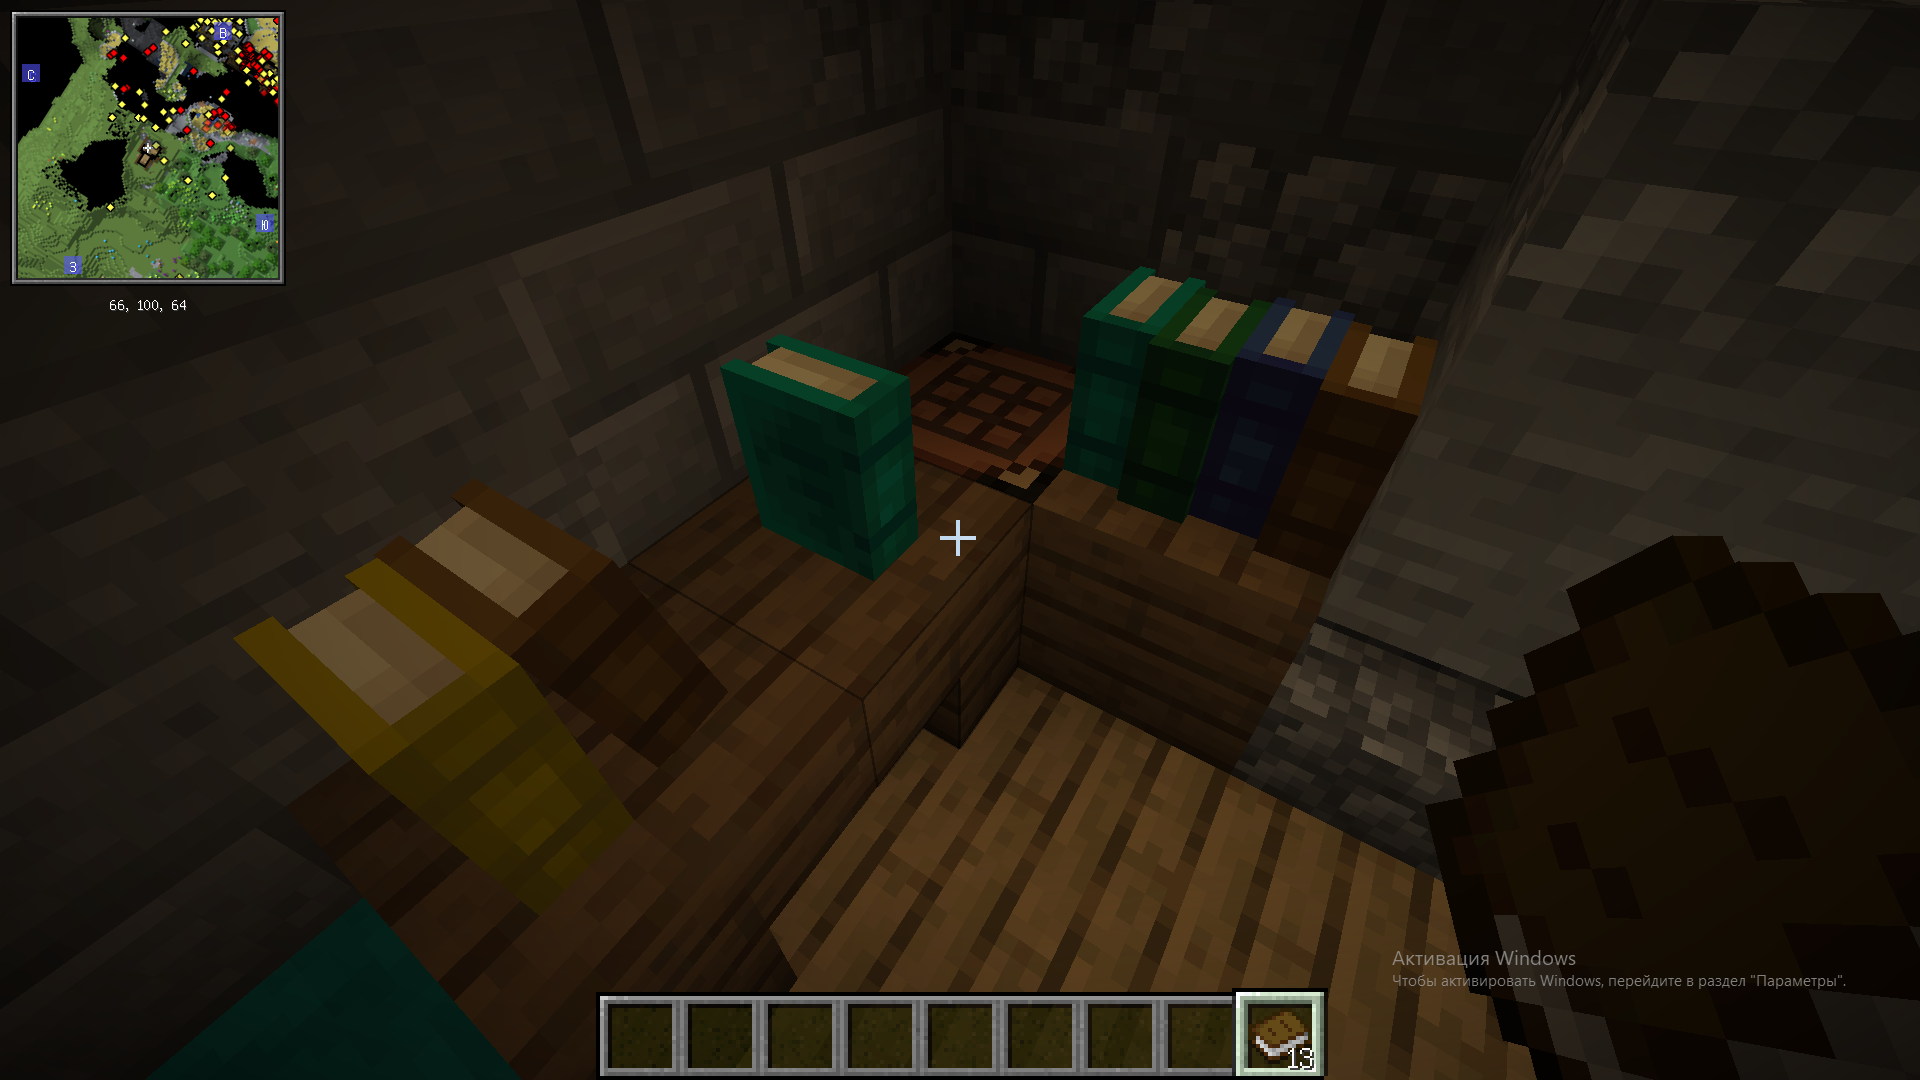
\includegraphics[width=6cm]{minecraft}

\end{center}

\section{Характеристика задачі}

ІС призначенна для автоматизації визначення закупки та підтримки прийняття рішеннь по цій темі. Вихідна інформація системи призначена для споживання менеджерами підприємства, та дає  можливість їм грунтовніше приймати рішення. Персонал що працює з системою може використовувати її в будь-який час для отримання результатів за найбільше декілька хвилин роботи сучасного комп'ютера.

Інформаційна модель

\section{Вихідна інформація}

Вихідна інформація ІС: 

\begin{enumerate}
	\item Варіанти оптимальної закупки
	\item Спрогнозована величина непередбачених витрат
	\item Дати початку замовленнь щоб виповнити план по даті старта виробництва
\end{enumerate}

Деталі в таблиці відповідно номерам:

{\small
\begin{center}
\begin{tabular}{ | c | c | c | c | c | }
\hline
 № з/п  & Ідентифікатор & Форма подання & Допустимий час затримки & Користувачі інформації \\ 
\hline
 1 & TODO & Веб сторінка & 1-2 минути & Кінцевий користувач \\  
\hline
 2 & TODO & Веб сторінка & 1-2 минути & Кінцевий користувач \\  
\hline
 3 & TODO & Веб сторінка & 1-2 минути & Кінцевий користувач \\  
\hline
\end{tabular}
\end{center}
}

\section{Вхідна інформація}

Вхідна інформація ІС: 

\begin{enumerate}
	\item Відомості про використання сировини на тех процессі
	\item Введення цільових показників продуктивності
	\item Запити на оптимальну закупку
	\item Запит на розрахунок непередбачених витрат
	\item Введення інформацію про поставки сировини
\end{enumerate}

Деталі в таблиці відповідно номерам:

{\small
\begin{center}
\begin{tabular}{ | c | c | c | c |  }
\hline
 № з/п  & Ідентифікатор & Форма подання & Джерело \\ 
\hline
 1 & TODO & Веб форма & Кінцевий користувач \\  
\hline
 2 & TODO & Веб форма & Кінцевий користувач \\  
\hline
 3 & TODO & Веб форма & Кінцевий користувач \\  
\hline
 4 & TODO & Веб форма & Кінцевий користувач \\  
\hline
 5 & TODO & Веб форма & Кінцевий користувач \\  
\hline
\end{tabular}
\end{center}
}

\section{Математичне забезпечення та алгоритм функціонування системи}

Задача оптимізації в ІС передбачае використання відповідних мат. методів. Обраний математичний метод - симплекс метод.

TODO: diagram 19.701—90 «Схеми алгоритмів, програм даних і систем. Умовні позначення і правила виконання».


